% -*- coding: utf-8 -*-
% !TEX encoding = UTF-8 Unicode
% !TEX root =  main.tex

\chapter{Theoretische und begriffliche Grundlagen}\label{cha:grundlagen}

Um auf die Regelung einer anisotropen Synchronmaschine einzugehen, werden im folgenden einige Grundlagen erörtert.

\section{Theorie der Drehfeldmaschinen}\label{sec:grund-drehfeld}

Drehfeldmaschinen sind die am häufigsten eingesetzten Antriebsmaschinen, der Grund hierfür ist die Robustheit der aktiven Bauteile und die gute Energieeffizienz.
Zudem besitzen Drehfeldmaschinen ein großes Leistungsspektrum und einen großen Drehzahl- und Drehmomentstellbereich.
Die wesentlichen Vertreter der Maschinenfamilie sind die Synchron- und die Asynchronmaschinen.
Beide basieren auf der Wirkung eines Drehfeldes, das sich durch den Luftspalt der Maschine bewegt.
Die Synchron- und Asynchronmaschine besitzen im Ständer denselben Aufbau und erfordern zur Darstellung ihres Verhaltens eine Reihe gleicher physikalischer Begriffe.
Es ist zweckmäßig die Grundlagen der Synchronmaschine in einem eigenen Kapitel zu behandeln.
Dies gilt \insb für den Aufbau der Drehstromwicklungen sowie die Grundlagen zur Beschreibung von umlaufenden Durchflutungen und deren Felder.

\section{Magnetfelder}



\subsection{Strombelag}

Die örtliche und zeitliche Änderung von Magnetfeldern in elektrischen Maschinen wird durch die Anordnung der Leiter und die Art der Speisung bestimmt \autocite[S~199]{hofmann2013}.
Die räumliche Verteilung des Stromes wird durch den Strombelag bestimmt, der als $N\cdot I$ pro Länge des bewickelten Umfanges definiert ist.

Das Luftspaltfeld hat die zentrale Bedeutung und muss deshalb auch berechnet werden können.
Die Ursache für die Entstehung dieses Luftspaltfeldes sind die vom Strom durchflossenen Leiter in den Nuten des Stators.
Unter der idealisierten Annahme eines homogenen Feldverlaufs im Bereich der Nutöffnung (s.~h.~Abbildung~\ref{fig:nutquerfeld}) das Feld im Luftspalt vom Feld in der Nut getrennt.

\begin{figure}[!htb]
\centering
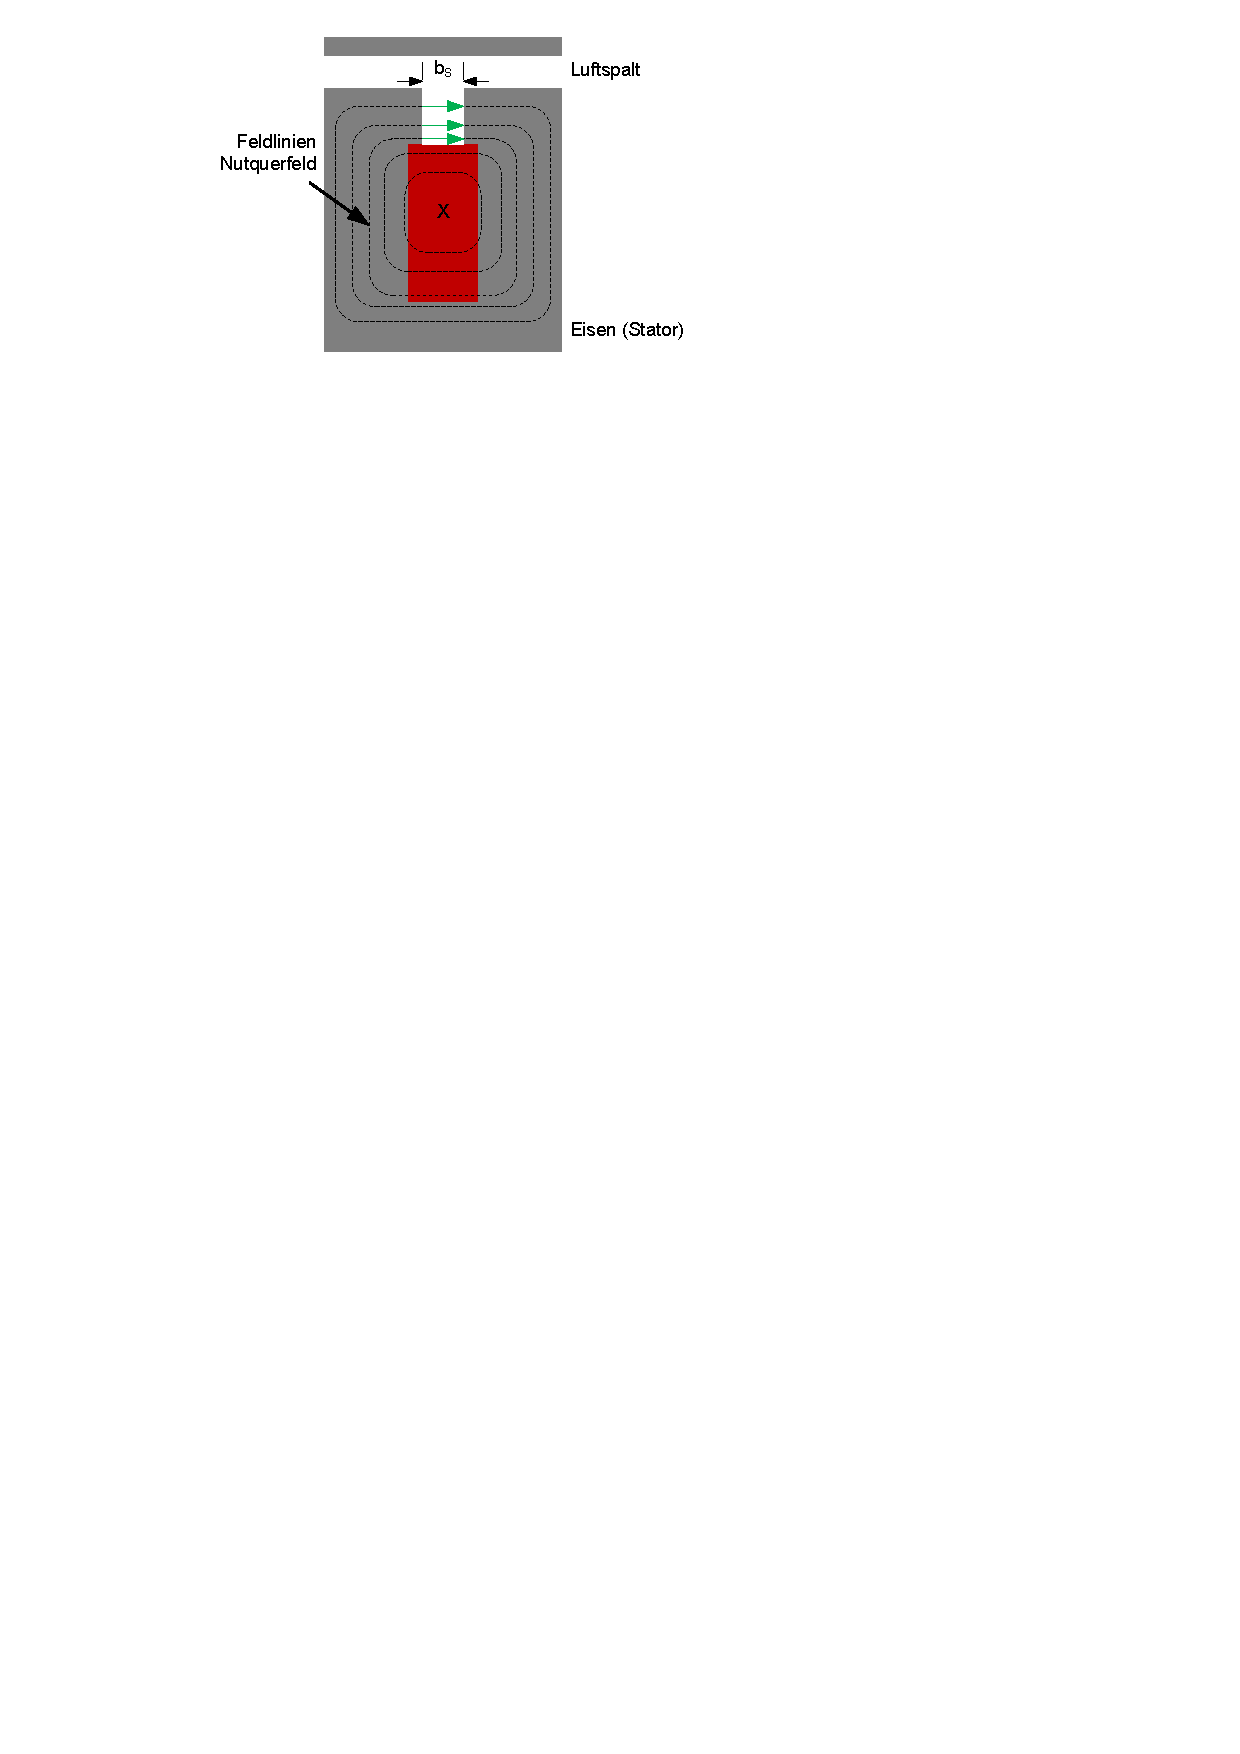
\includegraphics[width=\textwidth]{nutquerfeld.pdf}
\label{fig:nutquerfeld}
\caption{Abbildung des Nutquerfeldes einer Rechtecknut im Stator.}
\end{figure}

Hierzu wird die oben abgebildete Nut betrachtet, wobei die Permeabilität des Eisens als sehr groß gegenüber derjenigen von Luft angenommen wird ($\mu_\i{Fe} \rightarrow \infty$).
Es bildet sich ein Nutquerfeld aus, das ist leicht aus dem Durchflutungsgesetzt herzuleiten.

\begin{align}
\oint \vec{H}d\vec{l} = \Theta \label{eqn:durchflutungsgesetzt}
\end{align}

Dieses Nutquerfeld stößt an der Grenzfläche zwischen Nutöffnung (Nutschlitz bzw.\ Streuschlitz) und Luftspalt an das zu berechnende Luftspaltfeld und stellt somit eine der Randbedingungen zur Berechnung des Luftspaltfeldes dar.
Das Magnetische Feld in der Nutöffnung $H_\i{S}$, dass unter idealisierte Annahme tangential gerichtet ist, kann wiederum auch aus dem Durchflutungsgesetz berechnet werden.

\begin{align}
H_\i{S} = \frac{\Theta_\i{Nut}}{b_\i{S}}
\end{align}

Diese Randbedingung zur Berechnung des Luftspaltfeldes kann auch anders erzeugt werden.
Unter Annahme, dass die Nutdurchflutung $\Theta$ unendlich dünn auf einer glatten Eisenoberfläche gleichmäßig im Bereich der Nutöffnung $b_\i{S}$ verteilt ist.
Diese Modellvorstellung wird mit Hilfe des Strombelages beschrieben.

\begin{align}
A = \frac{\Theta_\i{Nut}}{b_\i{S}}
\end{align}

s.~h.~Abbildung~\ref{fig:strombelag-neu} zeigt die Modellvorstellung der obigen Beschreibung.

\begin{figure}[!h]
\centering
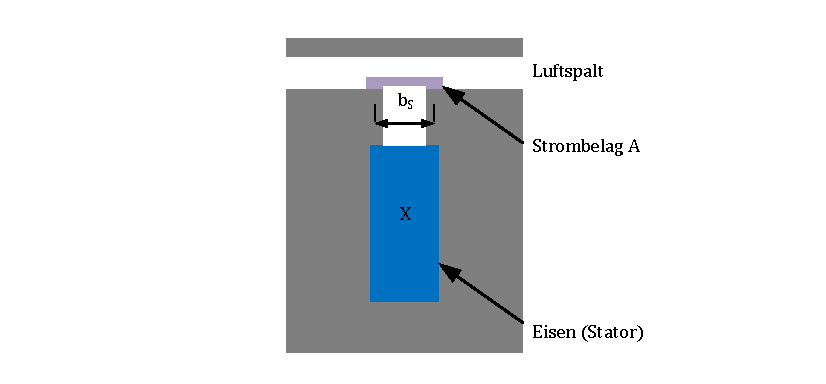
\includegraphics[width=\textwidth]{strombelag_neu.pdf}
\label{fig:strombelag-neu}
\caption{Vereinfachte Modellvorstellung zur Berechnung des Luftspaltfeldes mit Hilfe des Strombelags.}
\end{figure}

Bei Auswertung des Durchflutungsgesetz bei einem Umlauf um diesen Strombelag, ergibt sich für die tangentiale Feldstärke $H_\i{t}$ an der Eisenoberfläche im Bereich des Strombelages

\begin{align}
\oint \vec{H}d\vec{l} = \Theta_\i{Nut} \\
H_\i{t}\cdot b_\i{S} = A\cdot b_\i{S} \\
H_\i{t} = A = \frac{\Theta_\i{Nut}}{b_\i{S}} \label{eqn:feld-ht}
\end{align}

Mit Abbildung~\ref{eqn:feld-ht} ist gezeigt, dass die Randbedingungen zur Berechnung des Luftspaltfeldes unverändert erhalten bleibt, wenn statt der in Nuten eingebrachten Leiter ein äquivalenter Strombelag auf der glatten Eisenoberfläche berücksichtigt wird (Die Wirkung der Nutdurchflutung wird hinreichend genau durch den über der Nutöffnung verteilten Strombelag beschrieben).
Zur Berechnung des Luftspaltfeldes muss also nun das Nutenfeld nicht berücksichtigt werden.
Zudem kann eine deutlich vereinfachte Geometrie zugrunde gelegt werden.

\begin{quote}
Die Begrenzungsflächen von Stator und Rotor können als glatt angenommen werden, was in Umfangsrichtung der Maschine konstanten Luftspalt und demzufolge auch einen kostanten magnetischen Luftspaltleitwert entspricht. (Gerling 2008, \emph{Elektrische Maschinen und Antriebe}. Bundeswehr Universität in München.)
\end{quote}

\subsection{Mehrphasensysteme}

Bei einpoliger Verbindung von $m$ Wechselspannungsquellen entsteht eine Schaltung, die $(m+1)$ Klemmen aufweist (s.~h.~Abbildung~\ref{fig:mehrphasen}).
Haben diese $m$ Wechselspannungsquellen dieselbe Kreisfrequenz $\omega$, so stellt die Schaltung die Spannungsquelle eines allgemeinen Mehrphasensystems dar.

\begin{figure}[!h]
\centering
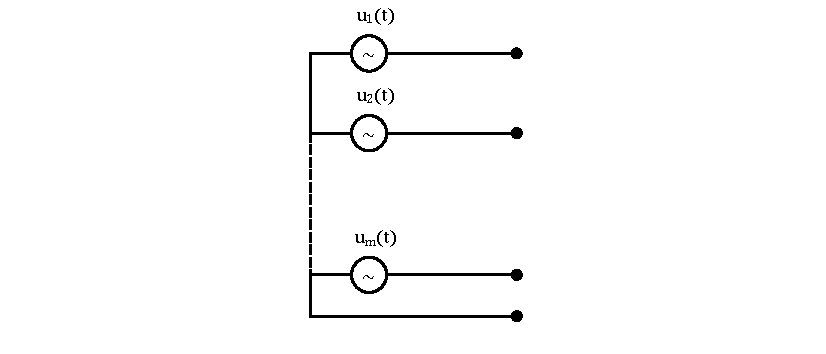
\includegraphics[width=\textwidth]{mehrphasen.pdf}
\label{fig:mehrphasen}
\caption{Spannungsquelle eines Mehrphasensystems.}
\end{figure}

Da keine Vorgaben bezüglich der Amplituden $\hat{u}$ und der Phasenlage $\varphi$ in der Definition der allgemeinen Mehrphasen-Spannungsquelle enthalten sind, kann sie \zB durch das folgende Gleichungssystemen beschrieben werden

\begin{align}
u_\i{1(t)} &= \hat{u}_\i{1} \cdot \cos(\omega t - \varphi_\i{1}) \\
u_\i{2(t)} &= \hat{u}_\i{2} \cdot \cos(\omega t - \varphi_\i{2}) \nonumber  \\
\vdots \nonumber \\
u_\i{m(t)} &= \hat{u}_\i{m} \cdot \cos(\omega t - \varphi_\i{m}) \nonumber
\end{align}

Aus der allgemeinen Mehrphasen-Spannungsquelle entsteht eine symmetrische Mehrphasen-Spannungsquelle, wenn zusätzlich gleiche Amplituden

\begin{align*}
\hat{u}_\i{1} = \hat{u}_\i{2} = \ldots \hat{u}_\i{m}
\end{align*}

und gleiche Phasenwinkeldifferenz zwischen aufeinanderfolgenden Teilspannungen gefordert werden

\begin{align*}
\varphi_\i{1} - \varphi_\i{2} = \varphi_\i{2} - \varphi_\i{3} = \ldots = \varphi_\i{m-1} - \varphi_\i{m} = \Delta \varphi
\end{align*}

Aus Symmetrieüberlegungen ergibt sich, dass die einheitliche Phasenwinkeldifferenz eine Funktion der Phasenzahl $m$ sein muss.

\begin{align}
\Delta \varphi = \frac{\omega T}{m} = \frac{2\pi}{m}
\end{align}

Darin tritt die Periodendauert $T$ der Teilspannungen auf.
Setzt man der Einfachheit

\begin{align*}
\varphi_\i{1} = 0
\end{align*}

so wird die symmetrische Mehrphasen-Spannungsquelle durch das folgende Gleichungssystem beschrieben.

\begin{align}
u_\i{1(t)} &= \hat{u} \cdot \cos(\omega t) \\ \label{eqn:drehstrom}
u_\i{2(t)} &= \hat{u} \cdot \cos(\omega t - \frac{\omega T}{m})\nonumber \\
\vdots \nonumber \\
u_\i{m(t)} &= \hat{u} \cdot \cos(\omega t - (m-1)\frac{\omega T}{m})\nonumber
\end{align}

In der Elektrotechnik treten Systeme mit verschiedenen Phasenzahlen auf.
Das Wechselstromsystem kann als Sonderfall des Mehrphasensystems mit $m=1$ aufgefasst werden.
Es kommt nur bei kleinen Leistungen zum Einsatz.
Eine Ausnahme stellt die Bahnversorgung dar, die bis zu großen Leistungen generell einphasig betrieben wird.
Gekennzeichnet ist diese durch die eingeprägte Frequenz von $f = 16\frac{2}{3}\mbox{Hz}$.

Die Phasenzahl $m=2$ tritt bei elektrischen Kleinmaschinen auf, allerdings nur in Form eines unsymmetrischen Systems mit einer Phasenwinkeldifferenz

\begin{align*}
\Delta \varphi = 90^{\circ} \,\text{bzw.\ } 270^{\circ}
\end{align*}

Die Phasenzahl $m=3$ kennzeichnet das Drehstromsystem, dass die Basis der elektrischen Energietechnik bildet.
Höhere Phasenzahlen treten \zB in der Stromrichtertechnik auf mit $m=6, 12, 24$.
Drehstromerzeuger mit Phasenzahl $m=3$ werden generell als symmetrisches System ausgelegt.
Als Klemmenbezeichnung ist die Buchstabengruppe $R, S, T$ bzw.\ $U, V, W$ üblich, wobei die gemeinsame Leitung der drei Teilspannungen mit $O, N$ oder $Mp$ für Mittelpunkt bezeichnet wird.

Durch die DIN-Normung wurde festgelegt, dass die Klemmenbezeichnung beim Drehstromsystem mit $L1, L2$ und $L3$ zu erfolgen hat.
Die Phasenwinkeldifferenz ist $\Delta \varphi = 120^{\circ}$.
Stellt man die Phasenspannungen $u_\i{1(t)}, u_\i{2(t)}, u_i{3(t)}$ nach Abbildung~\ref{eqn:drehstrom} dar, so ergibt sich 

\begin{figure}[!h]
\centering
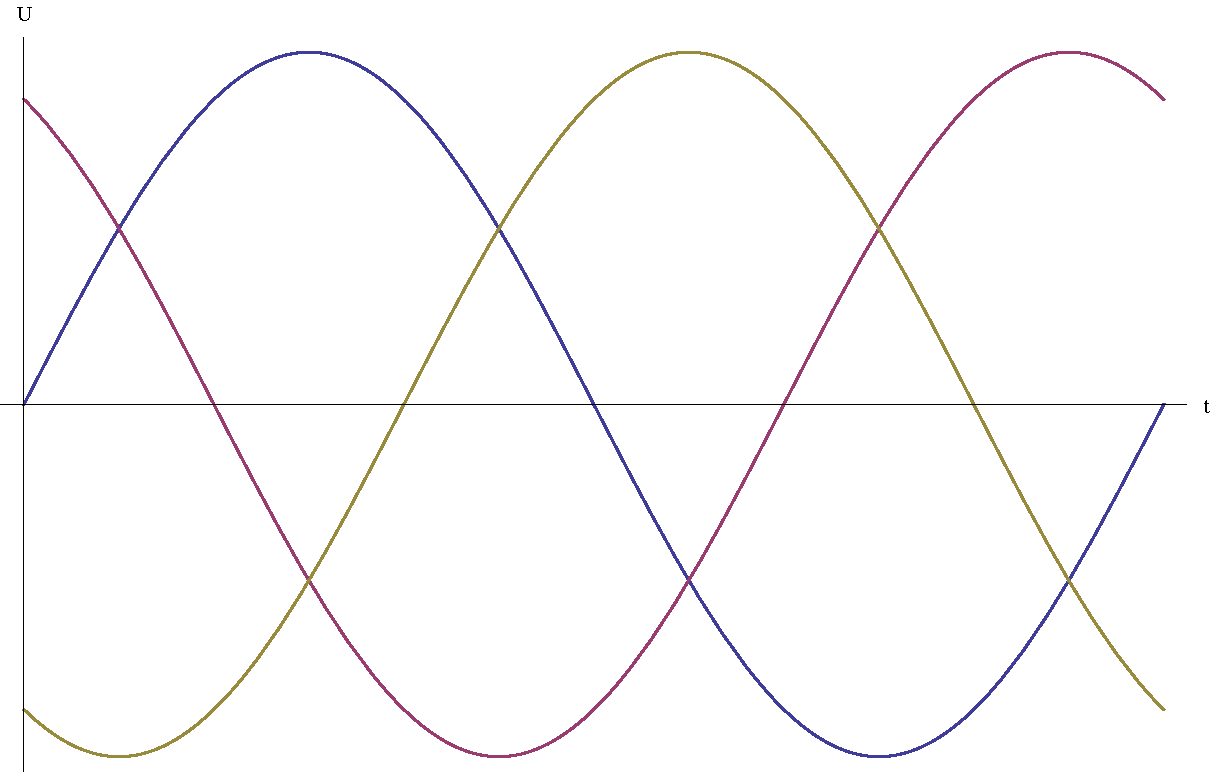
\includegraphics[width=\textwidth]{dreiphasensystem.pdf}
\label{fig:dreiphasen}
\caption{Phasenspannung eines symmetrischen Drehstromerzeugers.}
\end{figure}

Der prinzipielle Aufbau einer Drehstromwicklung lässt sich anhand aus den Anforderungen zur Erzeugung einer dreiphasigen Wechselspannung erläutern.
Eine solche Drehspannung erhält man mit einer Anordnung nach Abbildung~\ref{fig:drehstromwicklung}.
Ein aus Dynamoblechen geschichtetes Ständerblechpacket enthält in Nuten am Bohrungsumfang gleichmäßig verteilte Leiter, die zu drei räumlich verteilten Wicklungssträngen zusammengeschaltet werden \autocite[S.~141]{fischer2009}.
Der Läufer erzeugt ein Gleichfeld, das eine sinusförmige Feldverteilung längst des Luftspaltes aufbaut.
Hat der Läufer eine konstante Drehzahl, so induziert das Feld in den einzelnen Spulen zeitlich sinusförmige Spannungen, die sich innerhalb eines Wicklungsstranges zu einem Wert addieren.
Die Berechnung der Induktion kann über die Allgemeine Beziehung

\begin{align}
u_\i{q} = B\cdot l \cdot v
\end{align}

erfolgen.
Sei $d_1$ der Bohrungdurchmesser des Ständerblechpaketes einer $2p$-poligen Maschine, so bezeichnet man den Umfangsanteil

\begin{align}
\tau_\i{p} = \frac{d_\i{1} \cdot \pi}{2p}
\end{align}

wieder als Polteilung.
Die Polteilung entspricht der Länder einer Halbwelle der sinusförmigen Flussdichteverteilung im Luftspalt (enspricht einem elektrischen Winkel von $\omega t = 180^{\circ}$.
Bei einer zweipoligen Maschine mit $p=1$ stimmen somit der räumlich mechanische und der elektrische Winkel überein, allgemein gilt die Beziehung \autocite[S.141f.]{fischer2009}

\begin{align}
\gamma_\i{el} = p\cdot \gamma_\i{mech}
\end{align}

\begin{figure}[!htb]
\centering
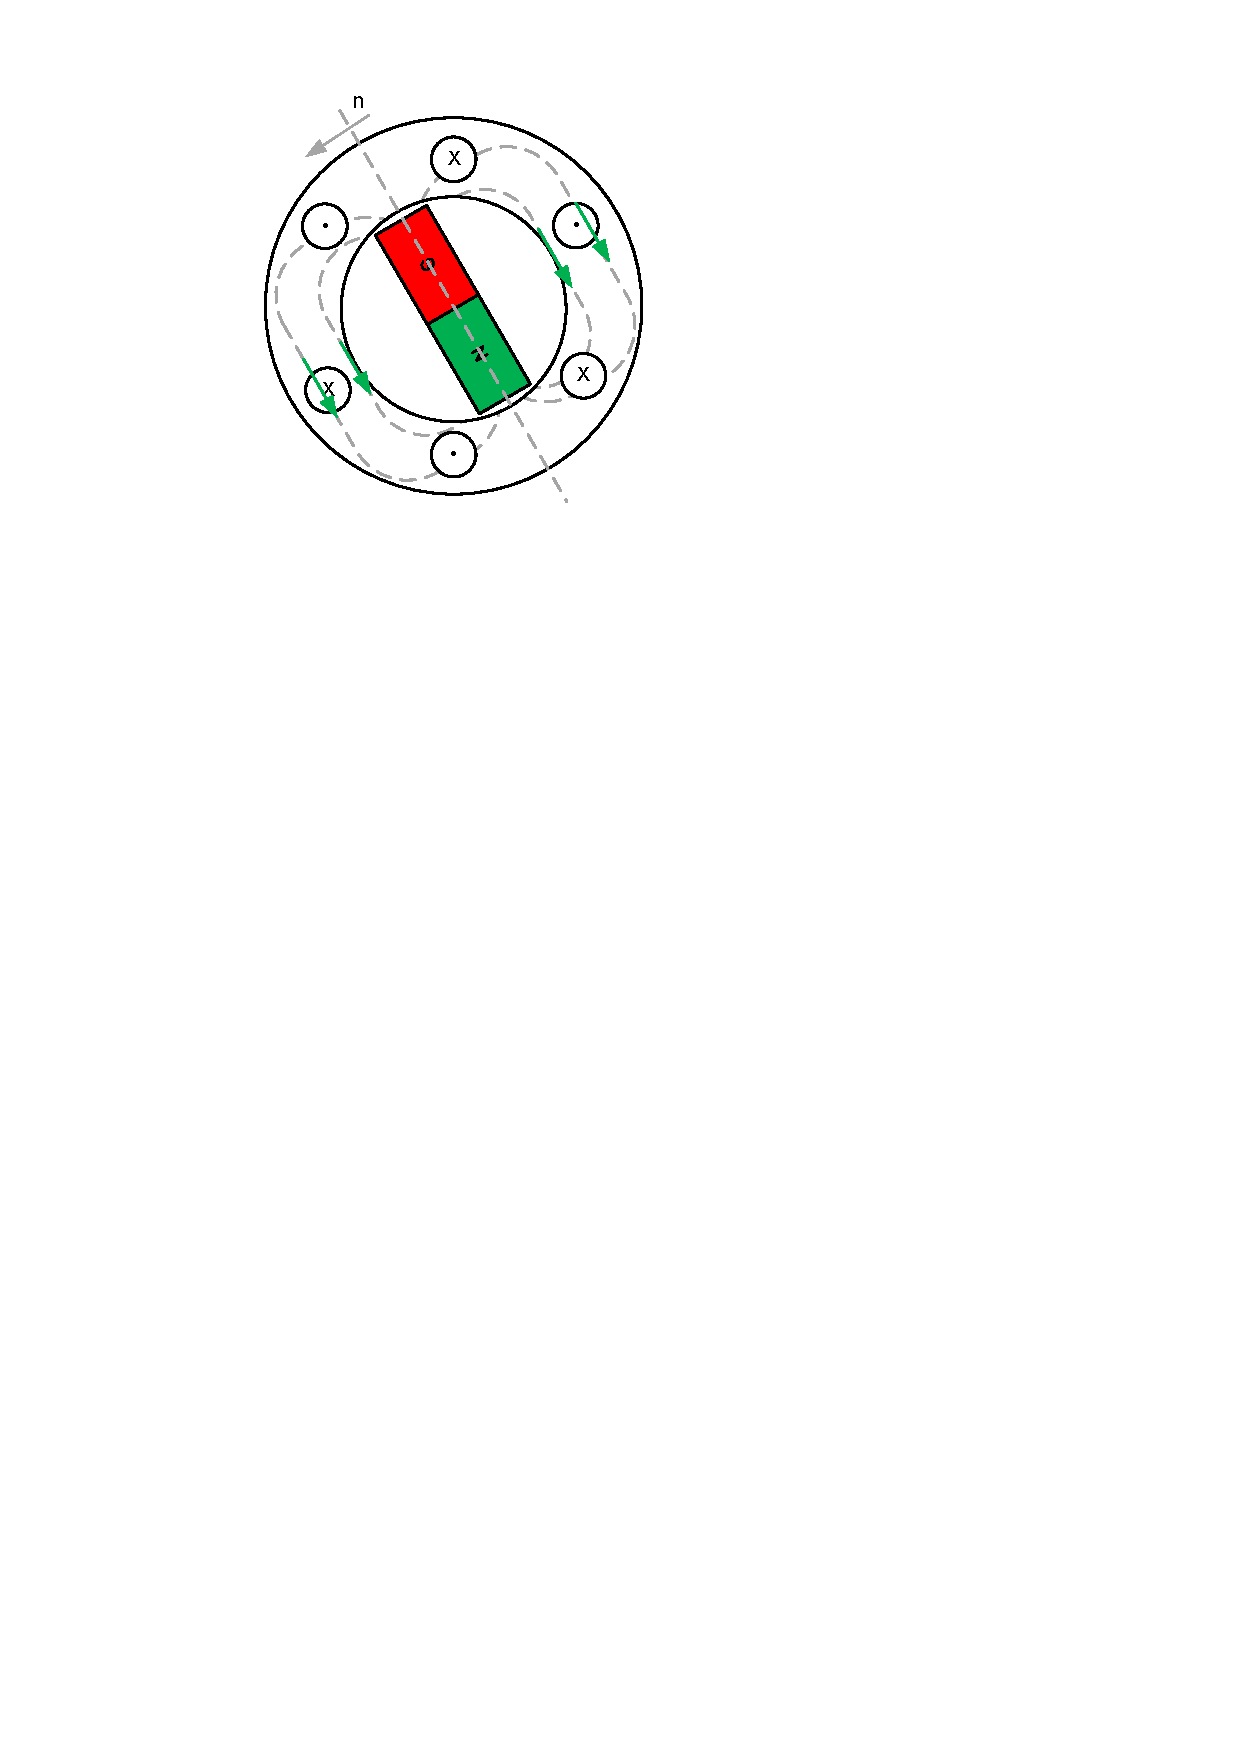
\includegraphics[width=\textwidth]{synchronmaschine-drehstrom.pdf}
\label{fig:drehstromwicklung}
\caption{Erzeugung einer mehrphasigen Spannung durch ein räumlich sinusförmiges Läuferdrehfeld.}
\end{figure}

\section{Induktivitäten}\label{sec:induktiv}

\section{Einführung Synchronmaschine}\label{sec:synchron}

\paragraph{Historischer Hintergund} Die ersten Synchronmaschinen wurden als Einphasengenerator entwickelt und gebaut, den ersten dreiphasigen Synchrongenerator entwickelten 1887 unabhängig voneinander F.~A.~Haselwander\footnote{Friedrich August Haselwander war ein deutscher Ingenieur, ein Erfinder der Drehstrom-Synchronmaschine und des kompressorlosen Ölmotors.} und C.~S.~Bradley\footnote{Charles Schenk Bradley war ein US-amerikanischer Elektrotechniker, Erfinder und Pionier von frühen Elektromotoren. Er zählt neben F.~A.~Haselwander zu den Begründern des heute im Bereich der elektrischen Energietechnik eingesetzten Dreiphasenwechselstromes.} Bei den Entwicklungen bildeten sich die Bauformen der Schenkelpol- und Vollpolmaschine aus. Die Weiterentwicklung der Synchronmaschine hing stark mit dem Ausbau der Energieversorgung und dem Bedarf von leistungsstärkeren Generatoren zusammen. Unabhängig von der Entwicklung wurden schon sehr früh Synchronmaschinen als Antriebsmaschinen für eine konstante Drehzahlregelung oder einen Phasenbetrieb in der Industrie eingesetzt \autocites[S.~287]{fischer2009}[S.~485f.]{mullerI2005}.

Die gleichstromgespeiste Erregerwicklung ermöglicht es, das Magnetfeld unabhängig vom Netz zu beeinflussen.
Als Spannungsquelle für die Speisung der Erregerwicklung wurden sog.\ Gleichstromerregermaschinen eingesetzt, in der heutigen Zeit werden Wechselspannung mit Hilfe von Leistungselektronischen Schaltungen gespeist.
Um die Schleifringübertragung der Erregerleistung zu umgehen, werden schleifring- bzw.\ bürstenlose Erregersysteme realisiert \autocite[S.~108]{ternes2012}.
Als Motor wurden Drephasen-Synchronmaschinen schon bald für große Leistungen eingesetzt, \zB zum Antrieb von Pumpen und Verdichten \autocite[S.~486]{mullerI2005}.
Der Nachteil ist, dass die Drehzahl durch die Netzfrequenz festgelegt ist.
Die Synchronmaschine arbeitet unabhängig von der Belastung stets mit der durch die Netzfrequenz und die ausgeführte Polpaarzahl festgelegten synchronen Drehzahl.

Heute ist es möglich mit Hilfe eines Frequenzumrichters die Drehzahl der Synchronmaschine zu steuern.
Aus diesem Grund werden größere Gleichstrommaschinen durch drehzahlvariable Synchronmaschinen abgelöst.
Im Bereich kleinerer Leistungen wird anstelle der Gleichstromerregung eine Erregung durch Permanentmagnete eingesetzt.
Dabei verliert man die Beeinflussung des Erregerzustandes über den Erregerstrom, dafür erhält man eine elektrische Maschine die keine elektrische Verbindung zum Läufer erfordert.

\subsection{Spannungsgleichungen und Ersatzschaltbild}

Die Synchronmaschine mit Vollpolläufer ist wegen ihres konstanten Luftspaltes mathematisch leichter erfassbar, als die Synchronmaschine mit Schenkelpolläufer.
Als Grundlage für weitere Betrachtungen dient dieses mathematische Modell als Grundlage.
Weiterhin wird vereinbart, dass
\begin{itemize}
	\item quasistationärer Betrieb
	\item Verbraucherzählpfeilsystem
	\item rechtsgängige Spulen
	\item läuferfeste, komplexe Ebene
\end{itemize}

\begin{figure}[!h]
\centering
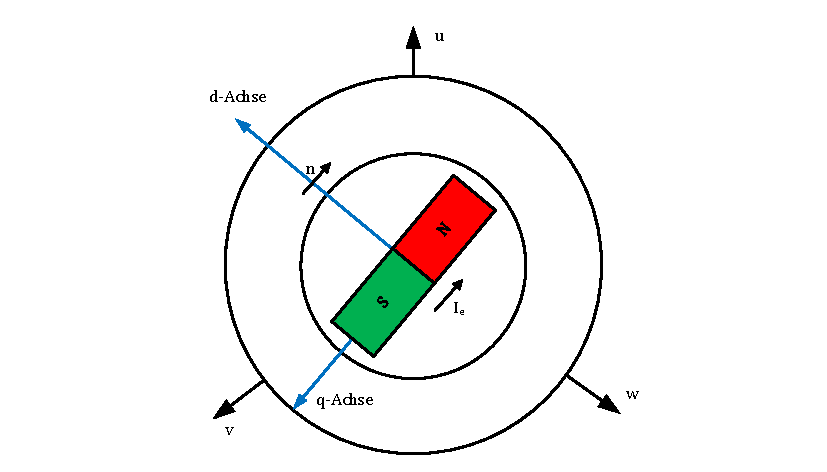
\includegraphics[width=\textwidth]{synchron-dq-1.pdf}
\label{fig:dq-synchron-1}
\caption{d,q-System der Synchronmaschine als Skizze.}
\end{figure}

\subsection{Beschreibung der Synchronmaschine im dq-Koordinatensystem}

Im folgenden wird angenommen, dass die Speisung des Polrads durch Permanentmagneten ersetzt wird.
In diesem Fall verbleiben nur die drei Statorwicklungen als stromdurchflossene Wicklungen.
Wesentlich bei den nachstehenden Überlegungen ist es, ob die Synchronmaschine als symmetrische Maschine (Vollpolläufer) oder als unsymmetrische Maschine (Schenkelpolläufer) konzipiert ist.
Die Wahl der Konzipierung hat Auswirkungen auf die Möglichkeit, Feldschwächebetrieb zu erreichen oder nur bedingt und dann mit Einschränkungen \autocite[S.~291]{schroder2000}.
Wird die Synchronmaschine in der Statorwicklung mit einer sinusförmigen Spannung versorgt, so ist diese als (PMSM) permanentmagneterregte Synchronmaschine definiert.
Bei einer trapezförmigen Speisung der Statorwicklung wird die Maschine als (BLDC) bürstenlose Gleichstrommaschine bezeichnet.
Der einfachste Fall für die Ermittlung des Signalflussplanes ist die Annahme, dass die Maschine an der Statorwicklung eine sinusförmige Spannung anliegt und die Maschine symmetrisch konzipiert wurde.
Bei einer symmetrisch konzipierten Synchronmaschine werden die Reluktanzeinflüsse nicht wirksam.
Damit ergeben sich nach \autocite[S.~291]{schroder2000} folgende Gleichungen für die Synchron-Vollpolmaschine.

\begin{align}
\frac{d\psi_\i{d}}{dt} &= U_\i{d} - R_\i{1}\cdot I_\i{d} + \Omega_\i{L}\cdot\psi_\i{q} \\
\frac{d\psi_\i{q}}{dt} &= U_\i{q} - R_\i{1}\cdot I_\i{q} + \Omega_\i{L}\cdot\psi_\i{d} \\
\end{align}

mit 

\begin{align}
\psi_\i{d} &= \psi_\i{PM} + L_\i{d}\cdot I_\i{d}\\
\psi_\i{q} &= L_\i{q}\cdot I_\i{q}
\end{align}

Damit ergibt sich das innere Luftspaltdrehmoment $M_i$ zu:

\begin{align}
M_\i{i} &= \frac{3}{2}\cdot Z_\i{p} \cdot (\psi_\i{d}\cdot I_\i{q} - \psi_\i{q}\cdot I_\i{d}) \\ 
\nonumber &= \frac{3}{2}\cdot Z_\i{p} \cdot (\underbrace{\psi_\i{PM}\cdot I_\i{q}}_\i{\text{~Hauptmoment}} + \underbrace{(L_\i{d}-L_\i{q})\cdot I_\i{d}\cdot I_\i{q}}_\i{\text{~Reluktanzmoment}}
\end{align}

und der allgemeinen mech.\ Bewegungsgleichung

\begin{align}
\Theta\cdot \frac{d\Omega_m}{dt} = M_\i{i} - M_\i{L}
\end{align}

\begin{figure}[!htb]
\centering
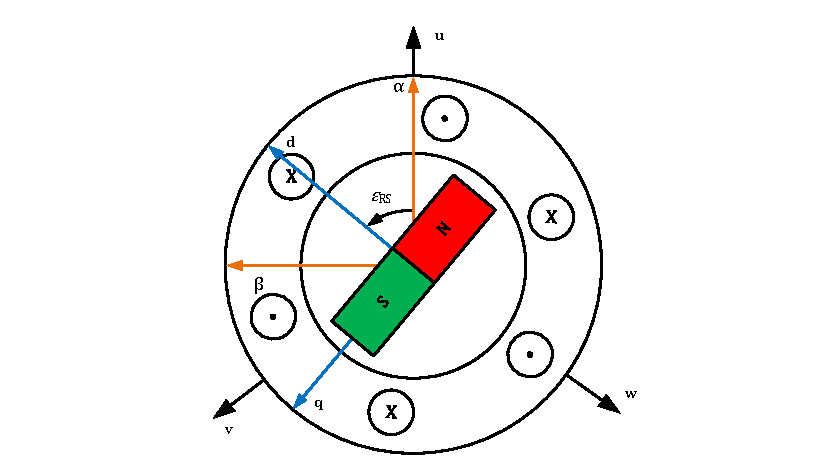
\includegraphics[width=\textwidth]{synchron-dq.pdf}
\label{fig:synchron-dq}
\caption{Darstellung der Synchronmaschine im dq-Koordinatensystem.}
\end{figure}

\section{Besonderheiten der Schenkelpolmaschine}\label{sec:schenkelpol}

\section{Permanenterregte Synchronmaschine}\label{sec:pmsm}

\section{Evalurierung der Ersatzschaltbilder für die Regelung}\label{sec:esb}

\begin{figure}[!htb]
\centering
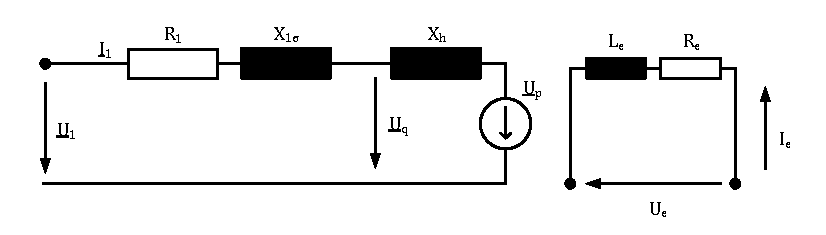
\includegraphics[width=\textwidth]{synchron-esb-kremser2004.pdf}
\label{fig:esb-kremser}
\caption{Ersatzschaltbild der Synchronmaschine nach \parencite[S.~145]{kremser2004}.}
\end{figure}

%%% Local Variables: 
%%% mode: latex
%%% TeX-master: "main"
%%% TeX-open-quote: "\\enquote{"
%%% TeX-close-quote: "}"
%%% LaTeX-csquotes-open-quote: "\\enquote{"
%%% LaTeX-csquotes-close-quote: "}"
%%% End: 

